\section{Kapitel 4: Wolken und Niederschlag}
\begin{tabular}{p{4cm} p{15cm}}
Aerosole	& \begin{tabular}[t]{lll}
		    Aitken-Kerne	& 0.01 - 0.1 $\mu$m	& $10^{10}$ / m$^3$\\
		    Grosse Kerne	& 0.1 - 2 $\mu$m	& $10^7$ / m$^3$\\
		    Riesen-Kerne	& 2 - 30 $\mu$m		& $10^6$ / m$^3$
		  \end{tabular}\\
Hydrometeoren	& \begin{tabular}[t]{lll}
		    \multicolumn{3}{p{14cm}}{Fl�ssige oder feste Bestandteile aus Wasser in der Atmosph�re. (Aerosole aus Wasser)}\\
		    Wolkentr�pfchen	& 0.001 - 0.2 mm	& $10^8$ / m$^3$\\
		    Regentropfen	& 0.2 - 8 mm		& $10^3$ / m$^3$\\
		    Hagelk�rner		& 8 - 100 mm		& 1 / m$^3$
		  \end{tabular}\\
Bedeutung der Aerosole	& Wichtig f�r Kondensation von Wasser und Bildung von Eis als Kondensations- bzw. Eiskeime\\
Beispiele f�r Aerosole	& Pollen, Russpartikel, Silikatpartikel (Sandsturm), Pilzsporen, Salzpartikel (Ozean, Gischt)\\
Prim�rpartikel		& Aerosol, das direkt von der Erdoberfl�che in die Atmosph�re gelangt.\\
Sekund�rpartikel	& Aerosol, das durch Nukleation (Partikelbildung aus Gasphase) entsteht.\\
Aitken-Kerne		& Entstehen haupts�chlich durch anthropogene Verbrennungsprozesse (Waldbr�nde, Industrie, Zigarettenrauch etc.)\\
Typische Konzentrationen von Aitken-Kernen	& \begin{tabular}[t]{lr}
                                          	  		& Mittel (cm$^{-3}$)\\\hline
							City	& 100'000\\
							Stadt	& 30'000\\
							Land	& 10'000\\
							Berg	& 1'000\\
							Ozean	& 400
                                          	  \end{tabular}\\
Trockene Deposition	& Die Aerosole fallen vom Himmel wegen der Gravitation oder der Brown'schen Bewegung (Diffusion)\\
Nasse Deposition	& Aerosole werden durch Wolkentr�pfchen oder sonstige Hydrometeoren eingefangen und aus der Atmosph�re entfernt.\\
L�sungstr�pfchen	& In Wasser l�sliche Aerosole. Eignen sich besonders gut f�r die Tr�pfchenbildung.\\
K�hler-Gleichung	& \begin{tabular}[t]{p{14cm}}
			      $\boxed{S = \frac{e'}{e_s} = 1 + \frac{a}{r} - \frac{b}{r^3}}$\\
			      $e'$: S�ttigungsdampfdruck von Wasser an der (krummen) Oberfl�che des L�sungstr�pfchens\\
			      $e_s$: S�ttigungsdampfdruck von Wasser �ber einer ebenen Oberfl�che\\
			      $r$: Radius des L�sungstr�pfchens\\
			      $a/r$: Kelvin-Effekt: S�ttigungsdampfdruck �ber krummer Oberfl�che ist geringer als �ber ebener Oberfl�che\\
			      $b/r^3$: Raoult-Effekt: S�ttigungsdampfdruck eines Wassertr�pfchens mit gel�sten Partikeln ist viel kleiner als eines reinen Wassertr�pfchens.
                	  \end{tabular}
\end{tabular}
\begin{tabular}{p{4cm} p{15cm}}
Niederschlagsbildung	& \begin{tabular}[t]{p{7cm}p{7cm}}
			  Warmer Regen				& Kalter Regen\\
			  1. Luft ist ges�ttigt (100\% RH)	& 1. 100\% RH und T $< 0^{\circ}$ C\\
			  2. Wolkentr�pfchen lagern sich an Aersolteilchen an	& 2. Eiskristalle werden gebildet durch Eiskeime (unterschiedl. Gefriertemperaturen)\\
			  3. Koaleszenz: Einzelne Wolkentr�pfchen kollidieren und bilden gr�ssere Wolkentr�pfchen (Regentropfen)	& 3. Schnelleres Wachstum, da $e_{s,Eis} < e_{s,Wasser}$
			  \end{tabular}\\
Gr�ssenverh�ltnisse	& \begin{tabular}[t]{llll}
			    Teilchen	& Radius ($\mu$m)		& Konzentration ($\tfrac{1}{\ell}$)	& Fallgeschwindigkeit ($\tfrac{cm}{s}$)\\\midrule
		Kondensationskeim	& 0.1				& $10^6$			& $10^{-4}$\\
		Wolkentr�pfchen		& 10				& $10^6$			& 1\\
		WT - RT Grenze		& 100				&				& 70\\
		Regentropfen		& 1000				& 1				& 650
			  \end{tabular}\\
Niederschlagspartikel	& Graupel, Flocken, Kristalle, Schneepartikel\\
Anheben eines bodennahen Luftpakets	& \begin{tabular}[t]{p{4cm}p{10.5cm}}
					    Gegeben	& Taupunktskurve ($T_d$), tats�chliche Temperaturkurve ($T$), Trockenadiabaten ($\theta$), Feuchtadiabaten ($\theta_e$), bodennahe H�he $h$\\
					    \textbf{Lifting condensation level (LCL)}	& Schnittpunkt ($\theta$ durch $T(h)$, $\theta_e$ durch $T_d(h)$) LCL = Wolkenbasis\\
					    \textbf{Level of free convection (LFC)}	& Schnittpunkt ($\theta_e$ durch LFC, $T$), wobei nach LFC $\theta_e > T \Rightarrow$ instabile Schichtung\\
					    \textbf{Level of neutral buoyancy (LNB)}	& Schnittpunkt ($\theta_e$ durch LFC, $T$), wobei nach LNB $\theta_e < T \Rightarrow$ stabile Schichtung
					  \end{tabular}\\
		& 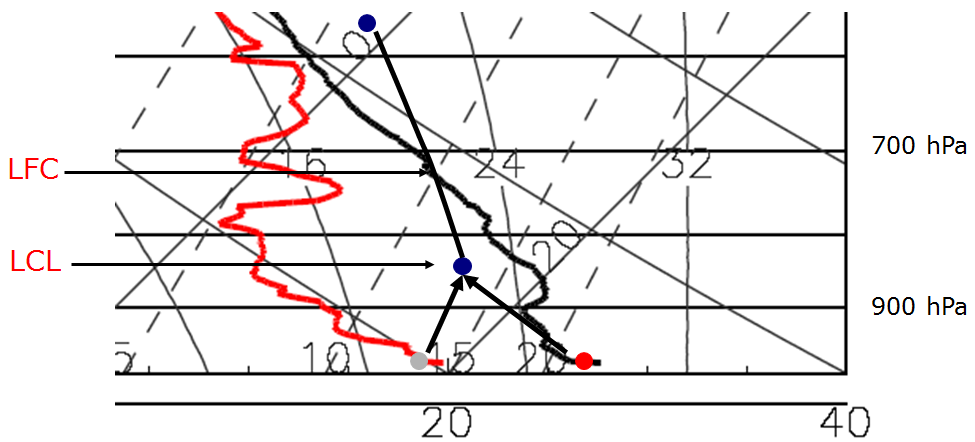
\includegraphics[width = 10cm]{atm_LCLLFC.png}\\
\end{tabular}

